\section{Introduction}
The baseline design of Cebaf Large Acceptance Spectrometer (CLAS12)\cite{nim:clas12} is composed of two tracking detectors: a Silicon Vertex Tracker (SVT) \cite{nim:svt} displayed in polyhedral 
arrangement around the target and sitting in a 5T-solenoid magnetic field to detect particles emitted between 40 and 130$^{\circ}$ with respect to the beam direction, as well as a forward tracker composed of drift chambers placed in a toroidal magnetic field for particles going between 5 and 35$^{\circ}$. 

In 2010, a proposal submitted by Irfu group for an upgrade of the baseline CLAS12 design was accepted by Jefferson Lab management. The upgrade of the central tracker consists in replacing the fourth layer of the SVT baseline design with 6 layers of cylindrical Micromegas detectors, called Barrel Micromegas Tracker (BMT). In addition, a Forward Micromegas Tracker (FMT) made of 6 Micromegas disks placed approximately 30~cm downstream of the target complete the drift chambers for forward tracking. FMT and BMT formed the Micromegas Vertex Tracker (MVT). Both tracking stations benefit from the specificities of both technologies as foreseen in early simulations and both offer improved resolutions for vertex and angle reconstructions compared to the baseline design. 

Together, the SVT and the BMT form the Central Vertex Tracker (CVT). The CVT is surrounded by two scintillator based detectors called Central Time-Of-Flight (CTOF) \cite{nim:ctof} and Central Neutron Detector (CND) \cite{nim:cnd} that provide particle identification information.

\section{System description}

\subsection{Micromegas detectors}
Micromegas detectors are micro-pattern gaseous detectors \cite{GIOMATARIS199629}. In a few-millimeter-wide conversion gap with an electric field of a few kV/cm, free electrons produced by the ionization of gas molecules by a charged particle are drifting towards an amplification gap. In the amplification gap, the electric field reaches several hundreds of kV/cm, accelerating the electrons arriving from the conversion gap and making them ionized the gas, creating consequently an electronic shower. The signal is then collected by readout strips.  

\begin{figure}[htb]
 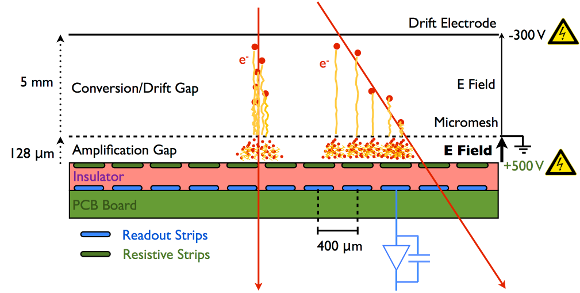
\includegraphics[width=1.0\columnwidth,keepaspectratio]{images/mm_principle}
 \caption{Schematic view of a resistive Micromegas detector.}
 \label{fig:mm-principle}
\end{figure}

The MVT must sustain the high particle flux which may induce sparks between the micromesh and the strips in nominal running conditions. In order to quench the sparks causing damages and temporary HV drop making the detector blind, all MVT detectors are based on the resistive techonology: as depicted by Fig.~\ref{fig:mm-principle}, resistive strips and a thin layer of insulator is deposited on top of the readout strips \cite{ALEXOPOULOS2011110}. The signals is transferred from resistive to readout strips by capacitive effect. Last but not least, resistive technology allows to reach gains higher than regular detectors and consequently increase the signal-over-background ratio. In this configuration the mesh is grounded and the high voltage for amplification is positive on the resistive strips. 

\subsection{General}

The Barrel Micromegas Tracker consists of six layers of cylindrical detectors, three with strips along the beam axis (Z strips) giving information about the azimuth angle of the particle and three with circular strips (C strips) perpendicular to the beam axis to constrain the polar angle. Each layer is made of three curved detectors covering 115$^{\circ}$. A total of 18 curved detectors are assembled on a carbon structure to complete the Barrel. In addition of the resistive technology, these detectors include the bulk technology, meaning that the micro-mesh is embedded with the pillars on top of resistive strips \cite{GIOMATARIS2006405}. The bulk technology enforces a uniform distance between the micromesh and the strips, maintaining consequently a uniform gain over the detector surface, despite the mechanical stress induced by the curvature of the tile.

\begin{figure}[htb]
 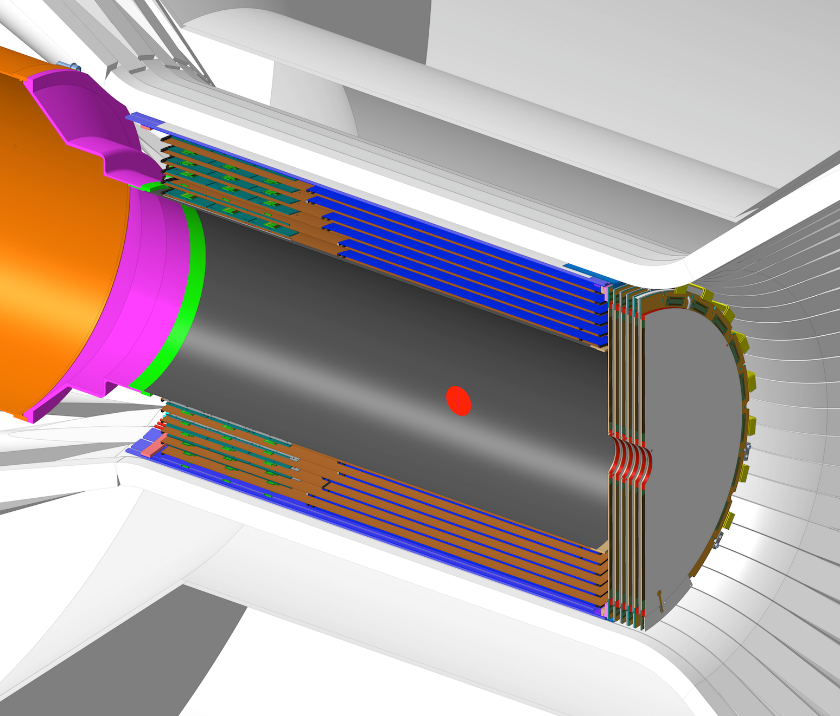
\includegraphics[width=1.0\columnwidth,keepaspectratio]{images/fig1}
 \caption{Cut view showing the 6 different layers of BMT and 6 identical FMT disks. It is shown inserted close to the central Time-of-Flight, itself in the 5T solenoid magnet. The SVT is inside the MVT and not displayed on this view.}
 \label{fig:mm-fig1}
\end{figure}

The Forward Micromegas Tracker consists of six flat Micromegas disks stacked together. The disks are all identical and assembled with a 60$^{\circ}$ rotation with respect to one another giving 3 angles of strips (0$^o$, 60$^o$ and 120$^o$). The resulting Micromegas Forward tracker is attached to the Barrel end flange. 

Figure \ref{fig:mm-fig1} displays a cut view showing all types of detectors for both BMT and FMT.

\subsection{Mechanical strucutre}
In order to hold the Micromegas Vertex Tracker in the magnet, a stainless-steel tube with the Barrel and Forward at its downstream end is attached to the flange of the SVT tube structure, as shown on Figure \ref{fig:mm-fig2}. This tube also holds 6 crates containing the 48 readout Front End Unit (FEU) boards for the Micromegas detectors as well as service distribution such as gas, enviromental sensors, and high-voltage distribution. The connection between detectors and readout FEU is done using assembled micro-coaxial cables allowing the signals readout from the distanced electronics crate. Each FEU is connected to Back End Unit with an optical fiber. The patch panels for the gas and the high voltage cables are located on the 6 crates.

\begin{figure}[htb]
 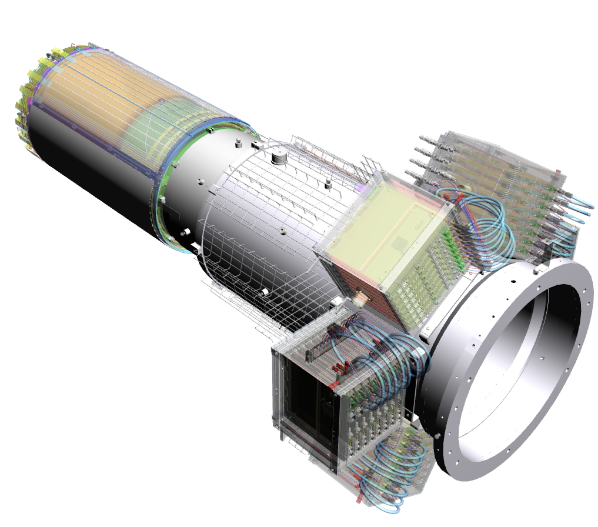
\includegraphics[width=1.0\columnwidth,keepaspectratio]{images/fig2}
 \caption{Support tube with electronics rack and MVT detectors.}
 \label{fig:mm-fig2}
\end{figure}

The mechanics of the Barrel structure is made of thin (1 mm) carbon cylinder with a glued PEEK flange downstream, and a glued stainless-steel flange upstream, as shown on Figure \ref{fig:mm-fig3}. Since the main purpose of the barrel is to reconstruct proton with momentum as low as 300~MeV, material budget must be as small as possible in order to reduce multiple scattering and energy loss.
The stainless steel used for the tube and flanges is made of 904L (non-magnetic steel). The alignment will be performed using particle tracks. A preliminary alignment is done using cosmic rays as described in a next section.

\begin{figure}[htb]
 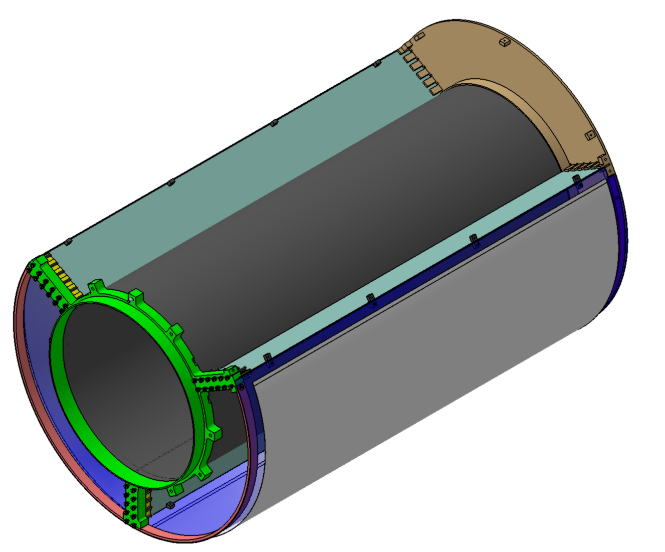
\includegraphics[width=1.0\columnwidth,keepaspectratio]{images/fig3}
 \caption{BMT mechanical structure, one sector open to house 6 curved detectors.}
 \label{fig:mm-fig3}
\end{figure}


\subsection{Barrel Micromegas Tracker (BMT)}

The Barrel detectors are made of a thin PCB (0.2 mm) transformed in Micromegas with the bulk process. Up to 16 MEC8 connectors 
are welded on the upstream side of the tile (upstream with respect to target position). The PCB is curved on a homemade mandrel tool with the desired radius. The cylindrical shape is then maintained by gluing two carbon fiber arches in under the active zone and two aluminum arches on the MEC8 connectors side. The carbon and aluminum structure thickness, 3 mm, defines the drift gap of the detectors. A Kapton foil (0.25 mm) with metallic coating is then glued on top of the carbon-aluminum structure to seal the detectors and be the drift electrode of the detector. A curved 3D-printed plastic mechanics is assembled above 
the connectors to provide rigidity for the connection of signal cables.  High voltage connections and the associated protection circuit are inside 4~cm $\times$ 8~cm metallic box on the side of the PCB.  Gas is introduced by the middle of the connector side and flush out on the edges of connector side through the hollow carbon-aluminum mechanical structure. The leak rate of each detector is measured bellow \(2\times10^{-3}\)~L/h.  On both ends of each carbon tube of the detectors are inserted and glued pin in order to fasten and localize the detectors to the barrel structure. Metrology has been performed on the assembled tiles and the radius error stays within 1 to 2 mm. Figure \ref{fig:mm-fig4} shows a view of curved BMT detectors.

\begin{figure}[htb]
 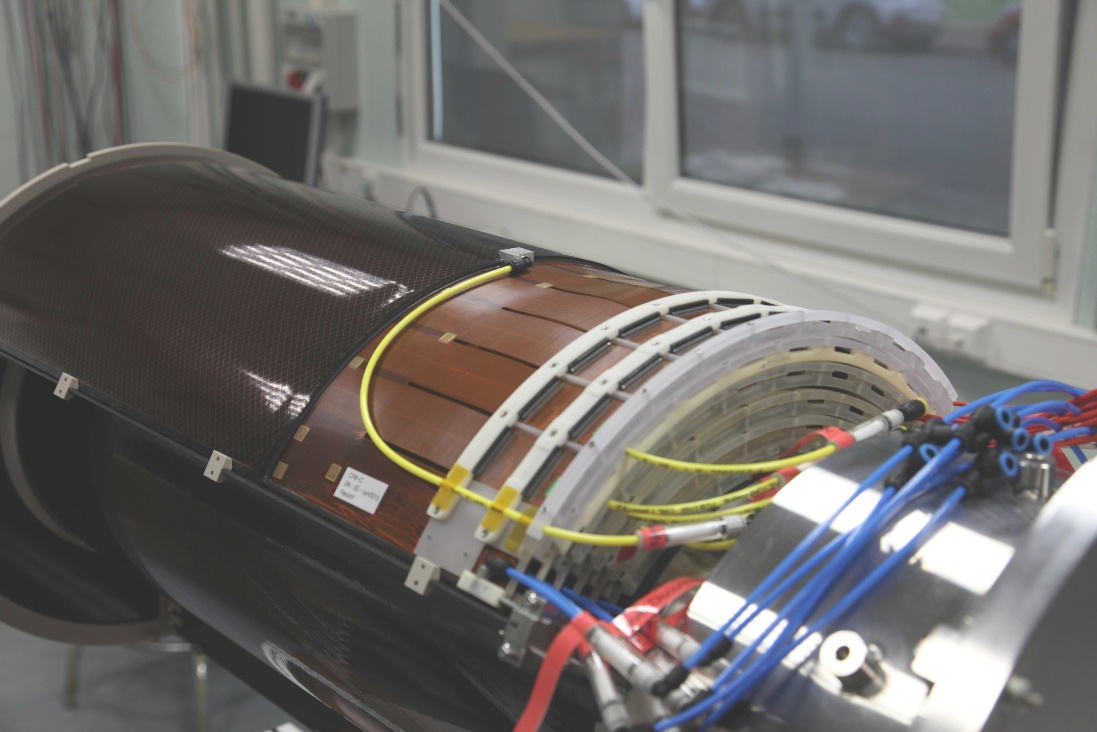
\includegraphics[width=1.0\columnwidth,keepaspectratio]{images/fig5}
 \caption{Full stack of 6 BMT layers in its mechanics.}
 \label{fig:mm-fig4}
\end{figure}

As pointed out before, the BMT is located inside the 5T solenoid used as a Moller shield. This situation had a strong consequence for the design and use of the BMT detectors: indeed, the (detector) electric and (solenoid) magnetic fields being essentially orthogonal, the primary electrons in the drift region of the Micromegas detectors are subject to a Lorentz angle, that make them drift transversally, therefore spreading the charge over a large area and directly impacting the position resolution and even the efficiency in extreme cases. Early studies by our group showed that strong Lorentz angles could be partly compensated by using a 5-6 kV/cm drift high voltage \cite{KONCZYKOWSKI2010274}. This increase of the drift field impact the efficiency through the loss of transparency by \(\approx5\%\). The effect is worst in the case of Z-type detectors with strips parallel to the B-field direction. Finally a gas mixture of 90\% Argon + 10\% isobutane offers a reasonable trade-off between a high number of electrons generated in the conversion gap thanks to a Penning effect in order to compensate the electron spread as well as a limited drift velocity to reduce the Lorentz force. 

\subsection{Forward Micromegas Tracker (FMT)}

The Forward Micromegas Tracker, shown in Figure 6 (middle), consists of six identical Micromegas resistive detectors in the forward region from 30 cm to 36 cm of the target center. Each Micromegas detector, shown in Figure 6 (left and right), is a 450 mm diameter disk with an active area of 1024 readout strips (525 $\mu$m pitch) in one projection. It consists of an assembly of two 0,2~mm PCB glued on a 2~mm Rohacell foam forming the 2~mm-thich readout plane and a 0,2~mm PCB for the drift plane glued on two cylindrical frames defining the gas volume. The inner frame is of made of PEEK ans the outer frame of aluminium. Both define the chamber and are attached to the readout plane using stainless steel screws. High voltage connections and associated filter circuits are diametrically located from one to the other on the side of the readout plane.
Signals are read out via 16 MEC8 connectors. The orientation of the strips from one disk to the next is rotated by 60 degrees. The distance between the readout strips of two consecutive disks is 10.5 mm. 

\begin{figure}[htb]
 
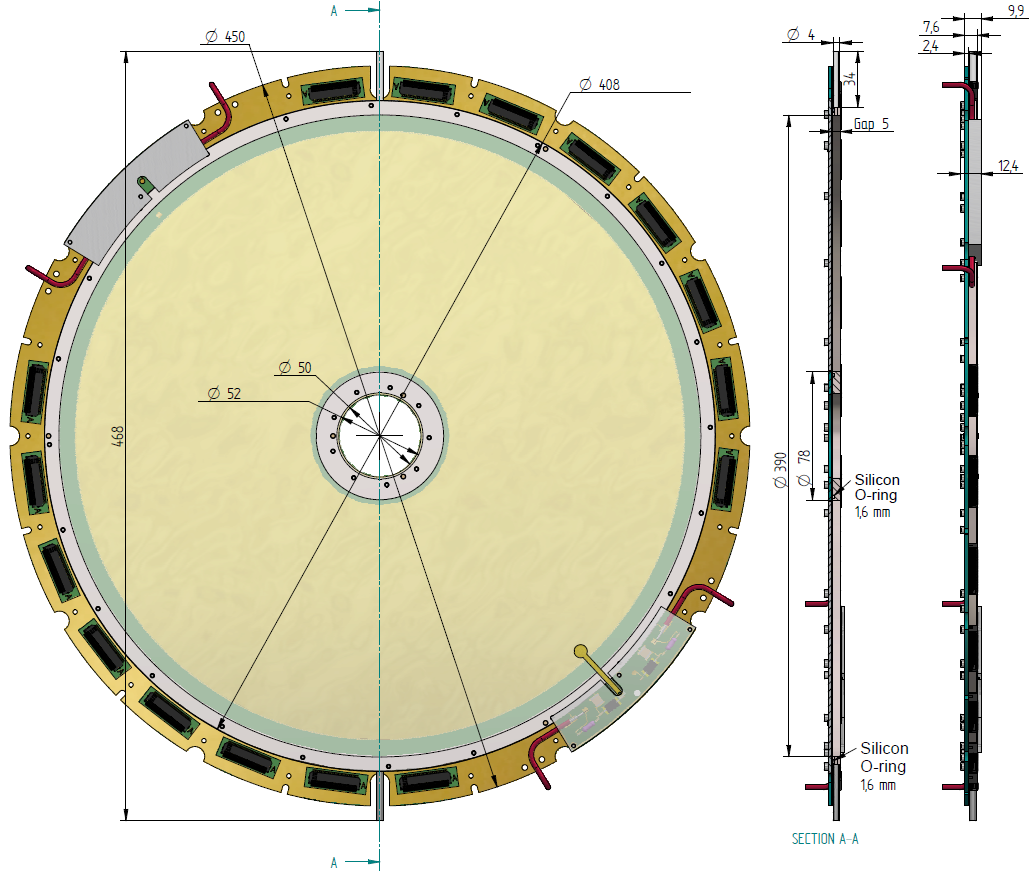
\includegraphics[width=0.66\columnwidth,keepaspectratio]{images/fig6_1}~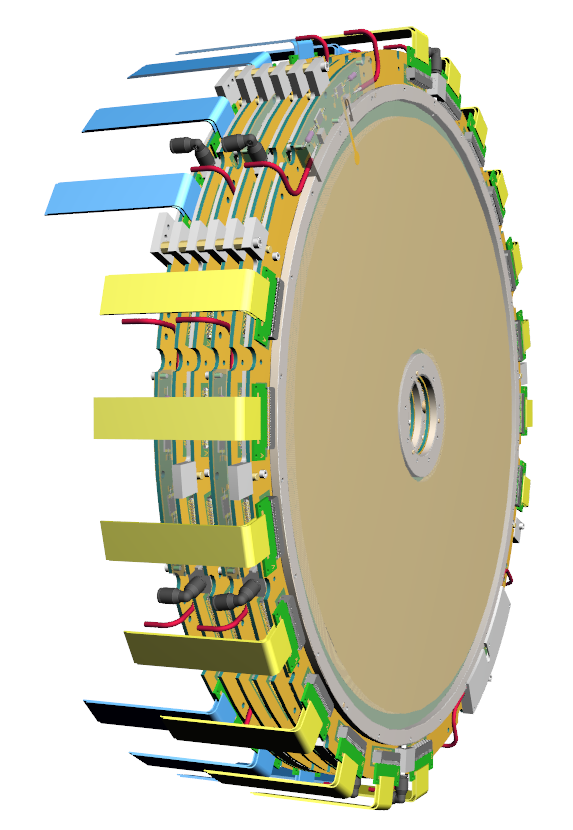
\includegraphics[width=0.33\columnwidth,
keepaspectratio]{images/fig6_2}
 \caption{CAD views of a FMT disks.}
 \label{fig:mm-fig5}
\end{figure}

By convention, the Micromegas detector are numbered from 1 to 6, (number 1 close to the target). The active area is divided in two parts, the inner part (IN),  diameter  $66 < d < 86$ mm, and the outer part (OUT), $168 < d < 380$ mm. 
In operation, a Micromegas detector has to be polarized by three high voltages (HV), the two active areas corresponding to the anode and the drift plane (cathode) 5 mm above the anode. The inner region can be disabled in case of pile-up (very high flux). Since the magnetic field is parallel to the drift field in the FMT, the Lorentz angle is no longer an issue but the high particle rate is. In order to improve timing resolution, a mixture of 80\% Argon + 10\% isobutane + 10\% CF$_4$ allows to increase the drift velocity compared to 90\% Argon + 10\% isobutane used in the BMT. 


\subsection{Gas system}
The Micromegas are continuously flushed with gas in order to keep a good purity and overcome the normal outgassing of the detectors. As stated in previous sections, the gas used for the barrel detector is a flammable mixture, argon with 10\% of isobutane. Each layer of the barrel is fed with one gas line, the tiles of a same layer being in serial, with a flow rate of about 1.5~L/h (liter per hour). For the FMT, the gas mixture is argon with 10\% of CF4 and 10\% of isobutane. The flow rate is 2~L/h for a set of three disks in serial. Thus a total of $\sim$ 13~L/h is requested for both FMT and BMT. No gas recirculation system has been designed for the MVT. 

\begin{figure*}[htb]
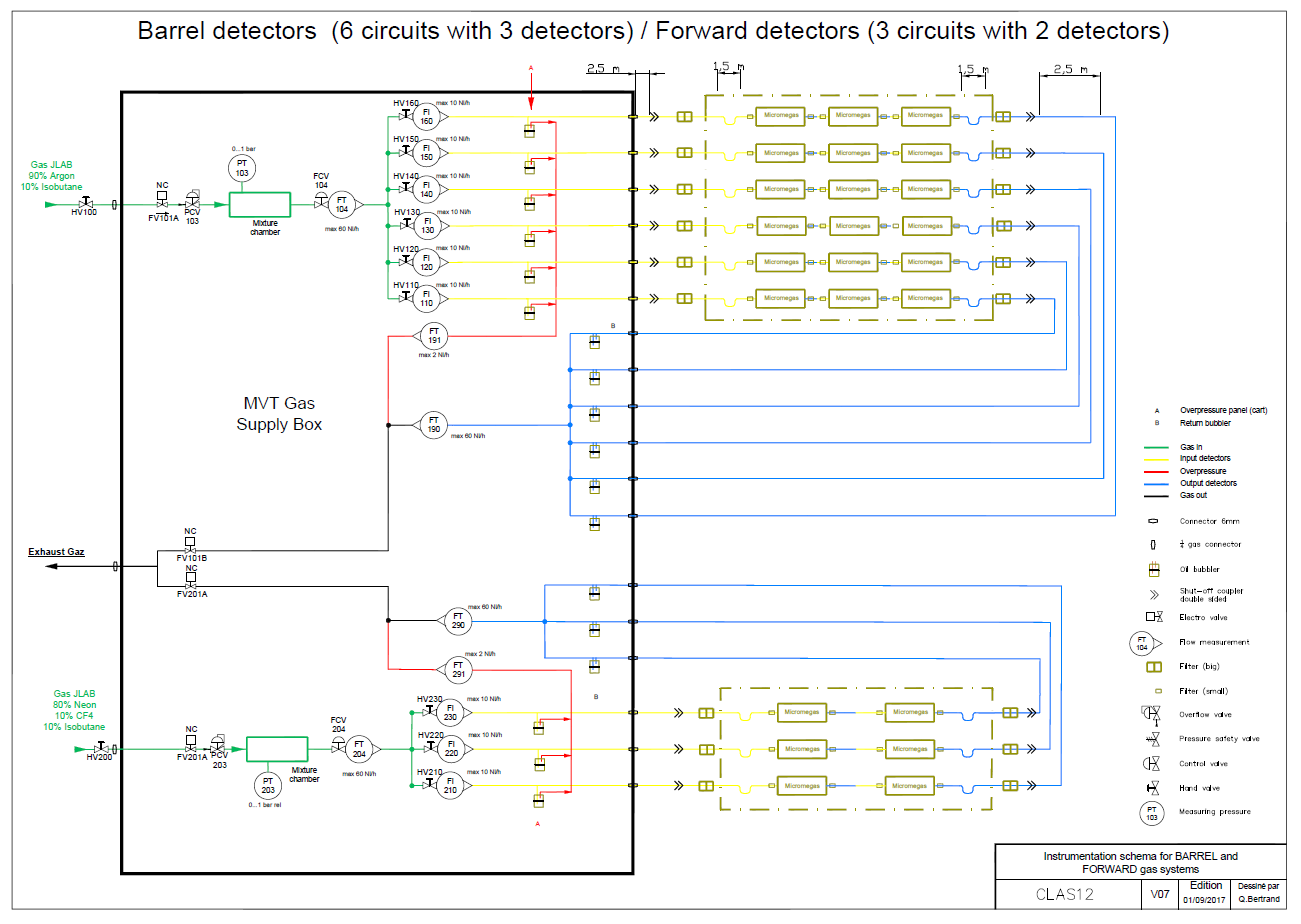
\includegraphics[width=2\columnwidth,keepaspectratio]{images/gas_system}
 \caption{Gas distribution diagram for the Micromegas vertex tracker.}
 \label{fig:mm-gas-sys}
\end{figure*}

A programmable logic controller controls the overall flow sent to the BMT and to the FMT which is provided by a gas mixing system located outside of the experimental hall. As shown in Figure~\ref{fig:mm-gas-sys}, a gas control panel then allows to adjust manually the gas distribution between the different lines for BMT and FMT. Inside the gas control panel, gas pressure and flow are measured at various points. The flow rate and pressure must indeed be low and controlled to avoid any deformation on the detectors. Interlocks are set to close valves and stop the gas flow in the detector if pressures or flows are above thresholds. 

Finally, total inflow and outflow are compared and trigger an interlock to stop the gas flow if in disagreement, hint of a leak in the systems. 

 